\documentclass[twocolumn]{article}

\usepackage{preprint}
\usepackage{graphicx}
\usepackage{tikz}
\usepackage{adjustbox}
\usepackage[most]{tcolorbox}
\usepackage{xcolor}
\usepackage{wrapfig}
\usepackage[hidelinks]{hyperref}
\usepackage{caption}
\usepackage{subcaption}

\title{Repeatable, Replicable, \& Reproducible experiments using OpenTTD}
\author{Michal Charemza}
\date{April 2023}

% From https://www.overleaf.com/latex/templates/sticky-notes/ftrvjddrmbwx
% Vebjørn S. Førde
% Creative Commons CC BY 4.0
% Yellow:
\definecolor{BgYellow}{HTML}{FFF59C}
\definecolor{FrameYellow}{HTML}{F7A600}
\newtcolorbox{YStkyNote}[1][]{%
    enhanced,
    before skip=2mm,after skip=2mm, 
    width=\columnwidth - 3mm, % width of the sticky note
    boxrule=0.2mm,
    colback=BgYellow, colframe=FrameYellow, % Colors
    attach boxed title to top left={xshift=0cm,yshift*=0mm-\tcboxedtitleheight},
    varwidth boxed title*=-3cm,
    % The titlebox:
    boxed title style={frame code={%
        \path[left color=FrameYellow,right color=FrameYellow,
        middle color=FrameYellow]
        ([xshift=-0mm]frame.north west) -- ([xshift=0mm]frame.north east)
        [rounded corners=0mm]-- ([xshift=0mm,yshift=0mm]frame.north east)
        -- (frame.south east) -- (frame.south west)
        -- ([xshift=0mm,yshift=0mm]frame.north west)
        [sharp corners]-- cycle;
        },interior engine=empty,
    },
    sharp corners,rounded corners=southeast,arc is angular,arc=3mm,
    % The "folded paper" in the bottom right corner:
    underlay={%
        \path[fill=BgYellow!80!black] ([yshift=3mm]interior.south east)--++(-0.4,-0.1)--++(0.1,-0.2);
        \path[draw=FrameYellow,shorten <=-0.05mm,shorten >=-0.05mm,color=FrameYellow] ([yshift=3mm]interior.south east)--++(-0.4,-0.1)--++(0.1,-0.2);
        },
    drop fuzzy shadow, % Shadow
    fonttitle=\bfseries, 
    title={#1}
}

\begin{document}

\twocolumn[
  \begin{@twocolumnfalse}
  
    \maketitle

    \begin{abstract}
        OpenTTD is an open source real time strategy (RTS) business simulation game based on the 1994 game Transport Tycoon Deluxe. In spite of being designed as a recreational game, OpenTTD has been the focus of a number of academic studies. However, these studies have problems regarding the repeatability, replicability, \& reproducibility of their experiments. This paper summarises the problems, and presents a simple framework that allows OpenTTD to be used in a way to avoid these problems in future research.
    \end{abstract}
\vspace{0.35cm}

  \end{@twocolumnfalse}
]

\section{Introduction}

OpenTTD \cite{openttd} is an open source real time strategy (RTS) simulation game. The aim of the game is to successfully run a business by constructing networks of roads, railways, airports and ports, along with their respective vehicles, trains, planes and ships, in order to transport people and goods in exchange for money. OpenTTD is played on a simulated landscape as can be seen in Figure \ref{fig:openttd}.

\begin{figure}[h]
\centering
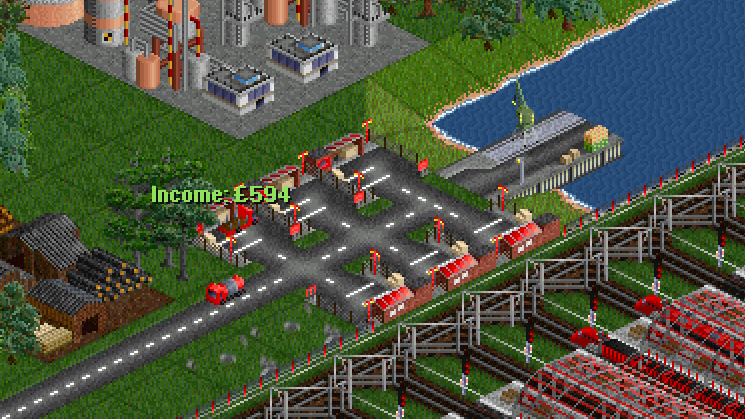
\includegraphics[width=\columnwidth]{assets/openttd-screenshot.png}
\caption{A small section of an OpenTTD (version 12.2) game at the moment when income is received for delivering goods by road. Also shown is part of a railway network, a port for ships, an oil refinery, and a sawmill.}
\label{fig:openttd}
\end{figure}

OpenTTD was created as a game for recreation. However, it is remarkably flexible: it has been successfully used as a tool to research artificial intelligence (AI) and machine learning (ML) algorithms \cite{wisniewski2011artificial, rios2009trains, bijlsma2014evolving}, scalability and mobile applications \cite{jiang2018mirroring}, and as a teaching aid \cite{HansenMuprhie2018}. It allows a single player to play in a non competitive world building mode, multiple human players playing cooperatively or competitively, and allows so-called custom AI-players that each control a company via code not part of the OpenTTD, but part of extensions to it written in the Squirrel language.

Using OpenTTD as a tool for research is the focus of this paper, and specifically its features for repeatable, replicable, \& reproducible research.

\section{Repeatability, Replicatability, \& Reproducibility}

The terms repeatability, replicability, and reproducibility unfortunately do not historically have universally agreed meanings \cite{plesser_reproducibility_2018}. To add to the confusion, the ACM have swapped their definitions reproducibility and replicability \cite{association_for_computing_machiner_new_2020}. For the avoidance of doubt, I use the ACM's definitions that are current as of October 2023 \cite{association_for_computing_machiner_artifact_2020}, summarised as

\begin{description}
\item[Repeatability] Same team, same artifacts
\item[Reproducibility]  Different team, using author-supplied artefacts
\item[Replicability] Different team, not using author-supplied artefacts
\end{description}

The strongest of these these, replicability, does not require a full re-implementation of all artifacts used in the research, but only those supplied by the author supplied. In OpenTTD terms, if an author writes a custom AI that is used in experiments, only that AI would need to be implemented by another team to replicate the research. OpenTTD itself would not need to be re-implemented. ? Say something about this... is this a limitation of the framework?

Beyond just supplying definitions, the ACM also provide a system of 5 badges \ref{fig:acm_badges} that can be applied to published research to incentivise research authors to make it so their research is reproducible and replicable by other teams. Other similar systems of badges are available, for example X, Y and Z.

"In each cases, exact replication or reproduction of results is not required, or even expected. Instead, the results must be in agreement to within a tolerance deemed acceptable for experiments of the given type. In particular, differences in the results should not change the main claims made in the paper."

\begin{figure}
     \centering
     \begin{subfigure}[b]{0.3\columnwidth}
         \centering
         
\includegraphics[width=\textwidth]{assets/artifacts_available.jpg}
         \caption{Artifacts available}
         \label{fig:y equals x}
     \end{subfigure}
     \hfill
     \begin{subfigure}[b]{0.3\columnwidth}
         \centering
         
\includegraphics[width=\textwidth]{assets/artifacts_evaluated_functional.jpg}
         \caption{Artifacts evaluated functional}
         \label{fig:three sin x}
     \end{subfigure}
     \hfill
     \begin{subfigure}[b]{0.3\columnwidth}
         \centering
         
\includegraphics[width=\textwidth]{assets/artifacts_evaluated_reusable.jpg}
         \caption{Artifacts evaluated reusable}
         \label{fig:five over x}
     \end{subfigure}
    \par\bigskip
     \begin{subfigure}[b]{0.3\columnwidth}
         \centering
         
\includegraphics[width=\textwidth]{assets/results_reproduced.jpg}
         \caption{Results reproduced}
         \label{fig:five over x}
     \end{subfigure}
     \begin{subfigure}[b]{0.3\columnwidth}
         \centering
         
\includegraphics[width=\textwidth]{assets/results_replicated.jpg}
         \caption{Results replicated  safd }
         \label{fig:five over x}
     \end{subfigure}
        \caption{The ACM system of badges for reproducble research}
        \label{fig:acm_badges}
\end{figure}

It is my hope that the framework presented here will make it more likely that research using OpenTTD will be not only repeatable, reproducible and replicable, but also more likely that upon publication, given all of these badges. ?? How often is the last one given - it surely requires a lot of effort

\section{Review of research using OpenTTD}

\begin{YStkyNote}
Give specific examples of the research and issues in research
\end{YStkyNote}

From the found published research using OpenTTD, in my opinion there is yet to be a single case that couldn't offer significant improvements in at least one of its repeatability, replicability or replicability.

Repeatability

Repeatability should be the easiest of the 3Rs to achieve, especially with computer based simulation. However, much of the existing research using OpenTTD uses a low number of repeated experiments, with little or no statistical analysis, suggesting that it was not straightforward.

Reproducibility

For reproducibility the author-supplied artifacts must be clear and available. There were references to modified OpenTTD in X,Y, no code of the custom AIs in X. Potentially the authors could be contacted to supply their own artefacts, but this is not ideal, nor offers a strong guarantee that the artefacts supplied were exactly as wthey were that generated the results.

No version of OpenTTD mentioned:
No author-supplied artefacts linked from paper
No mention of version of the author-supplied artefacts

Replicability

This is the most difficult to judge without actually attempting to do it.



\section{Review of OpenTTD command line options and configuration}
OpenTTD as of version 13.4 has over X command line options and Y configuration options that allow the player to customise how it behaves when playing. The ones that are particularly applicable to a  for repeatable, reproducible, and replicable research are reviewed below.

\subsection{Command line options}

\begin{description}
\item[-G \textless seed\textgreater] Allows the specification of the seed that initialises the random number generator that controls the pseudo random aspects of the game. For example, OpenTTD can auto generate landscapes. With the same seed (along with other configuration) one generation will be the same as the next
\item[-g] Starts a game immediately, rather than requiring the user to click through a introductory menu 
\item[-vnull:ticks=\textless number of ticks\textgreater] Puts the same into a "null" video mode that does not display the playing area on screen, and exits the game after a set number of \emph{ticks}. A tick is equal to approximately 1/Y of a day in game time.
\end{description}

The specification of the random seed should mean that OpenTTD affords exact repeatability and reproducibility when running as a simulation using only AI players. This means that it should be possible to make it straightfoward for to make results exactly reproducible, going beyond the requirements for ACM's badges on that front.

\subsection{Configuration options}

\begin{description}
\item[{fast\_forward\_speed\_limit} = \textless limit\textgreater] Limits the ticks per second the limit, which has a hard coded maximum in the game of 50000

\item[{[ai\_players]}] Allows the specification of which player are human and which are AI, and when they start playing.

\item[autosave = monthly|daily|other CHECK]

\item[keep\_all\_autosave]  A boolean value that allows all autosaves to be kept for further analysis
\end{description}

\section{Extracting data from OpenTTD}

OpenTTD saves its data in a custom binary format - its so-called savegame format. OpenTTD offers an extremely basic tool for extracting some data from this format, but it only shows X and Y. Since approxyimaty XXX a separate Python based tool has been available to extract data from save games

Extracting data from this format into a structure that is ready to be analysed has been done using. At the time of w

\section{Example results using these patterns}




\section{Possible extensions to OpenTTD}

Disable the max fast forward speed limit

Maximum number of autosaves

\begin{YStkyNote}
Suggest extensions that would address the issues of the research
\end{YStkyNote}

There are limited ways in which to extract data from the game.
Fast forward has a limit.
Can I be a spectator?

\section{Conclusion}

\begin{YStkyNote}
Briefly repeat the main points above
\end{YStkyNote}

\normalsize
\bibliographystyle{unsrt}
\bibliography{main}

\end{document}
